\section{决策部分}
\label{sec:policy}
\begin{frame}{决策部分}
    \begin{itemize}
        \item 输入:语义地图 (semantic map)
        \item 输出:
            \begin{itemize}
                \item 长期目标 (long-term goal)
                \item 当前行动 (action, path)
                \begin{itemize}
                    \item $a_t$: 向前,左转,右转,停
                \end{itemize}
            \end{itemize}
    \end{itemize}
    \note{
        \begin{itemize}
            \item 决策部分负责接受感知部分输出的语义地图
            \item 
            \item
        \end{itemize}
    }
\end{frame}


\begin{frame}{决策部分总体结构}
    \centering
    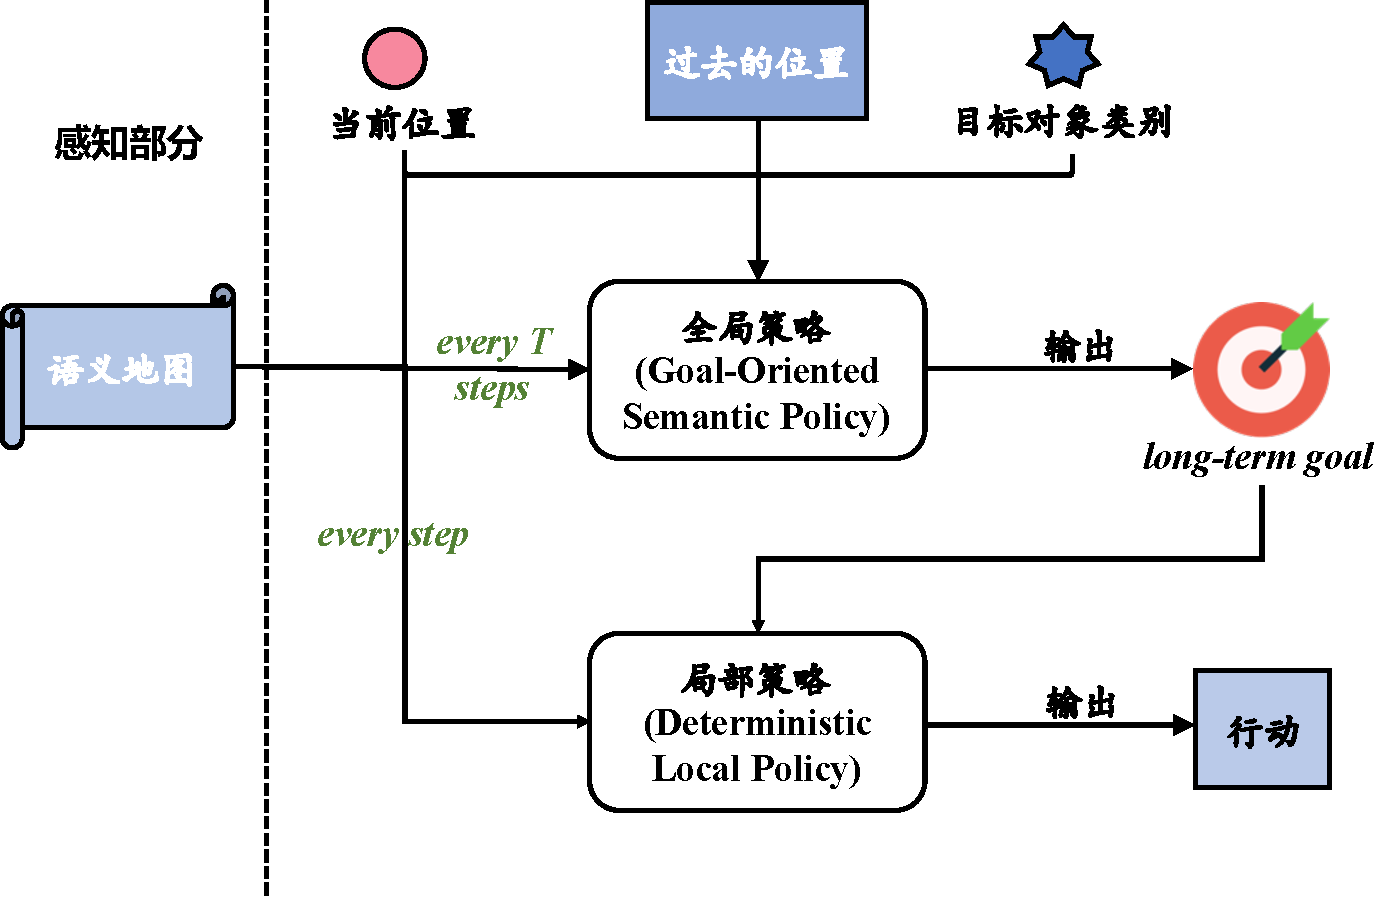
\includegraphics[width=11cm]{assets/policy_structure.pdf}
\end{frame}